\chapter{Implementation}

To demonstrate the feasibility of the proposed approach, a Java library for Android is developed. Also, a server application is developed for testing the library. The architecture is described on Figure \ref{fig:architecture}. Code for both the library and the server application is available in the project's repository \footnote[38]{https://github.com/huberflores/GestureMechanism, 14.05.15}.

\begin{figure}
\begin{center}
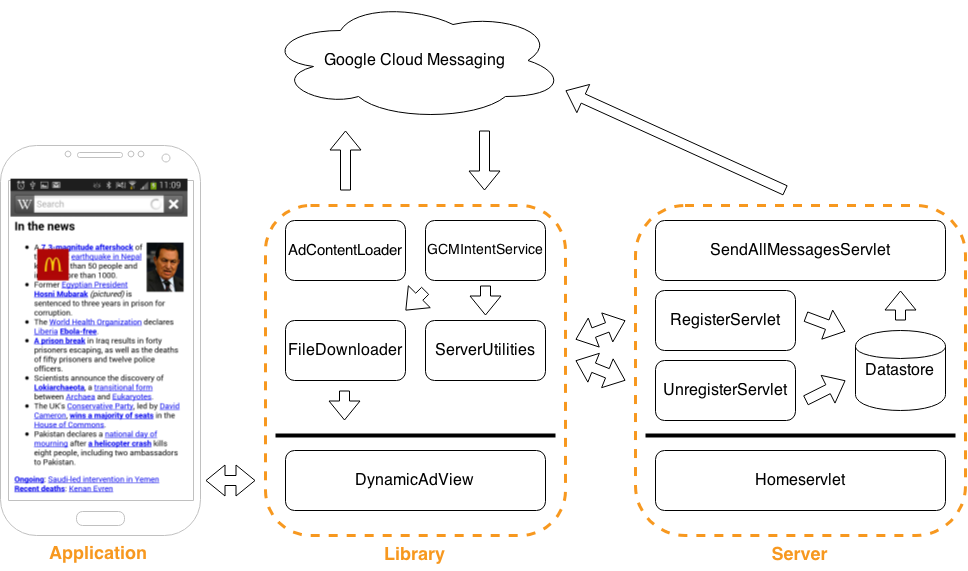
\includegraphics[scale=0.41]{Images/client-server.png}
\caption{Architecture of the developed mechanism}
\label{fig:architecture}
\end{center}
\end{figure}

\section{Application Library}

The library is a lightweight API that consists mainly of two parts: communication with the server,  and the ad view. The components of the server communication part are as follows:

\textbf{AdContentLoader} is the only class that the application developer should ever have the need to call. An instance of it is initialised in an activity's \textit{onCreate} method. It then adds the ad view to the activity's content view, registers a broadcast receiver to receive messages from the server and registers the device to Google Cloud Messaging service (GCM).\footnote[39]{http://developer.android.com/guide/google/gcm/, 14.05.15} The application developer should also call \textit{onPause} and \textit{destroy} methods in the activity's corresponding methods, the first of which unregisters from GCM and the second unregisters the broadcast receiver and disposes the GCM connection. The developer can also set the position of the appearing advertisement through this class.

\textbf{GCMIntentService} is a subclass of \textit{GCMBaseIntentService} and responsible for handling communication from GCM. It is based on Google Cloud Messaging, but could easily be adapted to fit another push notification framework, for example XMPP \cite{flores2013cloudmessaging}. \textit{onRegistered} method is called when the device is registered to GCM and makes a call to register to our back-end with the registration id from GCM. \textit{onUnregistered} unregisters the device from our back-end once it was unregistered from GCM. \textit{onMessage} receives and decodes the information about an advertisement that was sent from the server. There are also methods for receiving and handling server-side errors.

The \textbf{ServerUtilities} class is an abstraction layer for communicating with our server. It has methods for registering and unregistering the device that are called in \textit{GCMIntentService} as discussed previously.

Finally, \textbf{FileDownloader} is responsible for downloading the image files for an advertisement once \textit{GCMIntentService} receives and decodes them.

The user interface portion of the library is in a single class: \textbf{DynamicAdView}. It is responsible for the displaying the advertisement as well as handling the user's gestures. The view is invisible until \textit{FileDownloader} notifies \textit{AdContentLoader} that images for an advertisement have been downloaded. \textit{AdContentLoader} then prompts the view to update itself with the new images. The view is capable of handling pan, zoom and flick gestures. When the user moves the view out of the screen's bounds it remains invisible until another update notification.

\section{Back-end Distributor}

On the server-side there is a Java server application that handles the client's requests. The main components of the application are as follows:

\textbf{Datastore} is a simple implementation of a data store using standard Java collections. It is not persistent throughout redeploys, but its only purpose is to store the ids of registered devices.

\textbf{RegisterServlet} takes as a parameter the registration id from GCM and adds it to \textit{Datastore}'s id list. Likewise, \textit{UnregisterServlet} takes as a parameter the registration id from that a device is registered with and removes it from \textit{Datastore}'s id list.

\textbf{HomeServlet} is the only servlet with a graphical user interface. It has a label displaying the amount of registered devices as well as buttons to send pre-determined advertisements to the registered devices.

\textbf{SendAllMessagesServlet} is responsible for sending a push notification to each of the registered devices once a button in \textit{HomeServlet} is pressed. It takes as a parameter the id of an advertisement and based on that builds a GCM message which it then sends to all registered devices, tracking whether sending the message was successful or not and then returning to \textit{HomeServlet}

\section{API Integration into Mobile Lifecycle}

The Application Programming Interface (API) to use in an Android application is very minimalist. It's usage is explained in the project's repository \footnote[40]{https://github.com/huberflores/GestureMechanism/blob/master/README.md, 14.05.15}. To add the functionality of the mechanism to an application the developer has to import the Java archive file into the project. The \textit{AndroidManifest.xml} file of the application needs to be modified to include required permissions:

\lstset{language=XML}
\begin{lstlisting}
<permission
    android:name="your_package.permission.C2D_MESSAGE"
    android:protectionLevel="signature" />

<uses-permission android:name="your_package.permission.C2D_MESSAGE" />
<uses-permission android:name="com.google.android.c2dm.permission.RECEIVE" />
<uses-permission android:name="android.permission.GET_ACCOUNTS" />
<uses-permission android:name="android.permission.WAKE_LOCK" />
<uses-permission android:name="android.permission.INTERNET" />
<uses-permission android:name="android.permission.WRITE_EXTERNAL_STORAGE" />
<uses-permission android:name="android.permission.READ_EXTERNAL_STORAGE" />
<uses-permission android:name="android.permission.ACCESS_NETWORK_STATE" />
\end{lstlisting}

Also a broadcast receiver for Google Cloud Messaging notifications:

\begin{lstlisting}
<receiver
    android:name="com.in.mobile.gesture.ad.BroadcastReceiver"
    android:permission="com.google.android.c2dm.permission.SEND" >
    <intent-filter>
        <action android:name="com.google.android.c2dm.intent.RECEIVE" />
        <action android:name="com.google.android.c2dm.intent.REGISTRATION" />
        <category android:name="your_package" />
    </intent-filter>
</receiver>
\end{lstlisting}

and an intent service for Google Cloud Messaging:

\begin{lstlisting}
<service android:name="com.in.mobile.gesture.ad.GCMIntentService" />
\end{lstlisting}

Example usage of the mechanism in an activity would then look something like this:

\lstset{language=Java}

\begin{lstlisting}
import com.in.mobile.gesture.ad.AdContentLoader;
import com.in.mobile.gesture.ad.DynamicAdView.Position;

public class MyActivity extends Activity {

    AdContentLoader adLoader;

    @Override
    public void onCreate(Bundle savedInstanceState) {
        super.onCreate(savedInstanceState);

        // View code

        adLoader = new AdContentLoader(this);
        adLoader.setPosition(Position.TOP_RIGHT);
    }

    @Override
    public void onPause() {
        super.onPause();

        adLoader.onPause();
    }

    @Override
    public void onDestroy() {
        super.onDestroy();

        adLoader.destroy();
    }
}
\end{lstlisting}

\section{Summary}

A new mechanism which is less intrusive than conventional advertising frameworks was developed. As can be seen, the library is easy to use with any Android application. It relies on push notifications to display an advertisement on the device's screen. The simple back-end application can be used to demonstrate the proposed method of displaying advertisements to the user.

The next chapter discusses the method used for gathering user feedback and analyses the results to support the hypothesis that the proposed method improves user experience over conventional advertising methods.